\documentclass{beamer}
\usetheme{metropolis}
\usepackage{appendixnumberbeamer}
\usepackage{booktabs}

\usepackage{pgfplots}

% Presentation flow plan:
%
% Goals: 
%
%       0. Explain about my participation in the Kinetics challenge and the
%       stream fusion architecture idea that I came up with based on fusing
%       depth and motion (DeMoN) with RGB and pose networks.
%
%       The motivation of the current research is to extend the idea of stream
%       fusion to an automatic search over fusion operators.
%
%       The idea of presenting my work in this early stage is to request
%       feedback, ideas and direction from the group.
%
%
%       0. To what type of problems can fusion operator search be applied?
%
%       VQA: give MUTAN as motivation for improving performance by improving
%       the multi-modal fusion operator.
%
%       Action recognition in video: the "Revisiting the effectiveness of
%       off-the-shelf temporal modeling approaches for large-scale video
%       classification" Kinetics submission.
%
%       Take advantage of Dhanesh's multi-modal literature review:
%       SIGPROC-Rev1.pdf.
%
%
%       1-?. Present and explain the research on which my proposed research
%       depends.
%
%       1. Related, previous work on same topic from this group:
%
%       ModOut: https://hal.archives-ouvertes.fr/hal-01444614
%
%       Structure Optimization for Deep Multimodal Fusion Networks Using
%       Graph-Induced Kernels: https://arxiv.org/abs/1707.00750.
%
%
%       2a. Architecture search techniques:
%
%       Neural optimizer search with reinforcement learning:
%       http://proceedings.mlr.press/v70/bello17a.html.
%
%       Neural architecture search with reinforcement learning:
%       https://www.openreview.net/pdf?id=r1Ue8Hcxg.
%
%       Learning to learn by gradient descent by gradient descent:
%       https://arxiv.org/abs/1606.04474.
%
%
%       2b. Possible ways to apply architecture search to multi-modal fusion
%       problem.
%
%       Ask for ideas, based on what was just presented.
%
%       Ideas:
%               - Use dynamic programming to add layers, finding first the best
%               policy for a single fusion layer, then explore out to >= 2
%               layers.
%
%               In this case, the current state would be the state of the
%               fusion architecture that has been added on to the original
%               network, and the action space would be where to add the next
%               layer or fusion operation.
%
%               - Action space: join any of N activation map layers from each
%               stream with any other activation map using a fusion operator.
%
%               E.g., combine RGB and optical flow at multiple levels for
%               multiple parallel streams, and fuse those.

\title{Stream Fusion Operator Search}
\date{\today}
\author{Brendan Duke}
\institute{University of Guelph}

\begin{document}

\maketitle

\begin{frame}{Table of contents}
  \setbeamertemplate{section in toc}[sections numbered]
  \tableofcontents[hideallsubsections]
\end{frame}


\section{Introduction}

\begin{frame}{Stream fusion}
        \center{}
        \scalebox{.65}{
\definecolor{white}{RGB}{255,255,255}
\definecolor{cffda00}{RGB}{255,218,0}
\definecolor{cb26b00}{RGB}{178,107,0}
\definecolor{cff9900}{RGB}{255,153,0}
\definecolor{yellow}{RGB}{255,255,0}
\definecolor{cb28e00}{RGB}{178,142,0}
\definecolor{cffcc00}{RGB}{255,204,0}


\begin{tikzpicture}[y=0.80pt, x=0.80pt, yscale=-1.000000, xscale=1.000000, inner sep=0pt, outer sep=0pt,
draw=black,fill=black,line join=miter,line cap=rect,miter limit=10.00,line width=0.800pt]
  \begin{scope}[shift={(-474.0,27.0)},draw=white,fill=white]
    \path[fill,rounded corners=0.0000cm] (474.0000,-27.0000) rectangle
      (912.0000,405.0000);
  \end{scope}
  \begin{scope}[cm={{1.0,0.0,0.0,1.0,(-474.0,27.0)}},draw=cff9900,fill=cff9900]
    \path[fill,rounded corners=0.0000cm] (746.0000,48.0000) rectangle
      (776.0000,78.0000);
    \path[fill=cffda00,rounded corners=0.0000cm] (746.0000,48.0000) rectangle
      (747.0000,78.0000);
    \path[fill=cffda00,rounded corners=0.0000cm] (747.0000,48.0000) rectangle
      (775.0000,49.0000);
    \path[fill=cb26b00,rounded corners=0.0000cm] (747.0000,77.0000) rectangle
      (776.0000,78.0000);
    \path[fill=cb26b00,rounded corners=0.0000cm] (775.0000,48.0000) rectangle
      (776.0000,77.0000);
  \end{scope}
  \begin{scope}[cm={{1.0,0.0,0.0,1.0,(-474.0,27.0)}},line cap=butt,miter limit=1.45]
    \path[fill] (783.0615,67.1543) node[above right] (text4014) {Conv 1};
  \end{scope}
  \begin{scope}[cm={{1.0,0.0,0.0,1.0,(-474.0,27.0)}},draw=cff9900,fill=cff9900]
    \path[fill,rounded corners=0.0000cm] (746.0000,92.5000) rectangle
      (776.0000,122.5000);
    \path[fill=cffda00,rounded corners=0.0000cm] (746.0000,92.5000) rectangle
      (747.0000,122.5000);
    \path[fill=cffda00,rounded corners=0.0000cm] (747.0000,92.5000) rectangle
      (775.0000,93.5000);
    \path[fill=cb26b00,rounded corners=0.0000cm] (747.0000,121.5000) rectangle
      (776.0000,122.5000);
    \path[fill=cb26b00,rounded corners=0.0000cm] (775.0000,92.5000) rectangle
      (776.0000,121.5000);
  \end{scope}
  \begin{scope}[cm={{1.0,0.0,0.0,1.0,(-474.0,27.0)}},line cap=butt,miter limit=1.45]
    \path[fill] (781.8711,111.6543) node[above right] (text4030) {Max pool};
  \end{scope}
  \begin{scope}[cm={{1.0,0.0,0.0,1.0,(-474.0,27.0)}},draw=cff9900,fill=cff9900]
    \path[fill,rounded corners=0.0000cm] (746.0000,143.0000) rectangle
      (776.0000,173.0000);
    \path[fill=cffda00,rounded corners=0.0000cm] (746.0000,143.0000) rectangle
      (747.0000,173.0000);
    \path[fill=cffda00,rounded corners=0.0000cm] (747.0000,143.0000) rectangle
      (775.0000,144.0000);
    \path[fill=cb26b00,rounded corners=0.0000cm] (747.0000,172.0000) rectangle
      (776.0000,173.0000);
    \path[fill=cb26b00,rounded corners=0.0000cm] (775.0000,143.0000) rectangle
      (776.0000,172.0000);
  \end{scope}
  \begin{scope}[cm={{1.0,0.0,0.0,1.0,(-474.0,27.0)}},line cap=butt,miter limit=1.45]
    \path[fill] (787.0479,162.1543) node[above right] (text4046) {Block 1};
  \end{scope}
  \begin{scope}[cm={{1.0,0.0,0.0,1.0,(-474.0,27.0)}},draw=cff9900,fill=cff9900]
    \path[fill,rounded corners=0.0000cm] (746.0000,207.0000) rectangle
      (776.0000,237.0000);
    \path[fill=cffda00,rounded corners=0.0000cm] (746.0000,207.0000) rectangle
      (747.0000,237.0000);
    \path[fill=cffda00,rounded corners=0.0000cm] (747.0000,207.0000) rectangle
      (775.0000,208.0000);
    \path[fill=cb26b00,rounded corners=0.0000cm] (747.0000,236.0000) rectangle
      (776.0000,237.0000);
    \path[fill=cb26b00,rounded corners=0.0000cm] (775.0000,207.0000) rectangle
      (776.0000,236.0000);
  \end{scope}
  \begin{scope}[cm={{1.0,0.0,0.0,1.0,(-474.0,27.0)}},line cap=butt,miter limit=1.45]
    \path[fill] (787.0479,226.1543) node[above right] (text4062) {Block 2};
  \end{scope}
  \begin{scope}[cm={{1.0,0.0,0.0,1.0,(-474.0,27.0)}},draw=cff9900,fill=cff9900]
    \path[fill,rounded corners=0.0000cm] (746.0000,260.5000) rectangle
      (776.0000,290.5000);
    \path[fill=cffda00,rounded corners=0.0000cm] (746.0000,260.5000) rectangle
      (747.0000,290.5000);
    \path[fill=cffda00,rounded corners=0.0000cm] (747.0000,260.5000) rectangle
      (775.0000,261.5000);
    \path[fill=cb26b00,rounded corners=0.0000cm] (747.0000,289.5000) rectangle
      (776.0000,290.5000);
    \path[fill=cb26b00,rounded corners=0.0000cm] (775.0000,260.5000) rectangle
      (776.0000,289.5000);
  \end{scope}
  \begin{scope}[cm={{1.0,0.0,0.0,1.0,(-474.0,27.0)}},line cap=butt,miter limit=1.45]
    \path[fill] (787.0479,279.6543) node[above right] (text4078) {Block 3};
  \end{scope}
  \begin{scope}[cm={{1.0,0.0,0.0,1.0,(-474.0,27.0)}},draw=cff9900,fill=cff9900]
    \path[fill,rounded corners=0.0000cm] (746.0000,314.0000) rectangle
      (776.0000,344.0000);
    \path[fill=cffda00,rounded corners=0.0000cm] (746.0000,314.0000) rectangle
      (747.0000,344.0000);
    \path[fill=cffda00,rounded corners=0.0000cm] (747.0000,314.0000) rectangle
      (775.0000,315.0000);
    \path[fill=cb26b00,rounded corners=0.0000cm] (747.0000,343.0000) rectangle
      (776.0000,344.0000);
    \path[fill=cb26b00,rounded corners=0.0000cm] (775.0000,314.0000) rectangle
      (776.0000,343.0000);
  \end{scope}
  \begin{scope}[cm={{1.0,0.0,0.0,1.0,(-474.0,27.0)}},line cap=butt,miter limit=1.45]
    \path[fill] (787.0479,333.1543) node[above right] (text4094) {Block 4};
  \end{scope}
  \begin{scope}[cm={{1.0,0.0,0.0,1.0,(-474.0,27.0)}},draw=cffcc00,fill=cffcc00]
    \path[fill,rounded corners=0.0000cm] (631.0000,75.0000) rectangle
      (700.0000,96.0000);
    \path[fill=yellow,rounded corners=0.0000cm] (631.0000,75.0000) rectangle
      (632.0000,96.0000);
    \path[fill=yellow,rounded corners=0.0000cm] (632.0000,75.0000) rectangle
      (699.0000,76.0000);
    \path[fill=cb28e00,rounded corners=0.0000cm] (632.0000,95.0000) rectangle
      (700.0000,96.0000);
    \path[fill=cb28e00,rounded corners=0.0000cm] (699.0000,75.0000) rectangle
      (700.0000,95.0000);
  \end{scope}
  \begin{scope}[cm={{1.0,0.0,0.0,1.0,(-474.0,27.0)}},line cap=butt,miter limit=1.45]
    \path[fill] (851.4814,202.6543) node[above right] (text4110) {ResNet};
  \end{scope}
  \begin{scope}[cm={{1.0,0.0,0.0,1.0,(-474.0,27.0)}},draw=cffcc00,fill=cffcc00]
    \path[fill,rounded corners=0.0000cm] (645.0000,122.0000) rectangle
      (687.0000,143.0000);
    \path[fill=yellow,rounded corners=0.0000cm] (645.0000,122.0000) rectangle
      (646.0000,143.0000);
    \path[fill=yellow,rounded corners=0.0000cm] (646.0000,122.0000) rectangle
      (686.0000,123.0000);
    \path[fill=cb28e00,rounded corners=0.0000cm] (646.0000,142.0000) rectangle
      (687.0000,143.0000);
    \path[fill=cb28e00,rounded corners=0.0000cm] (686.0000,122.0000) rectangle
      (687.0000,142.0000);
    \path[fill,rounded corners=0.0000cm] (655.5000,169.0000) rectangle
      (676.5000,190.0000);
    \path[fill=yellow,rounded corners=0.0000cm] (655.5000,169.0000) rectangle
      (656.5000,190.0000);
    \path[fill=yellow,rounded corners=0.0000cm] (656.5000,169.0000) rectangle
      (675.5000,170.0000);
    \path[fill=cb28e00,rounded corners=0.0000cm] (656.5000,189.0000) rectangle
      (676.5000,190.0000);
    \path[fill=cb28e00,rounded corners=0.0000cm] (675.5000,169.0000) rectangle
      (676.5000,189.0000);
    \path[fill,rounded corners=0.0000cm] (655.5000,207.0000) rectangle
      (676.5000,228.0000);
    \path[fill=yellow,rounded corners=0.0000cm] (655.5000,207.0000) rectangle
      (656.5000,228.0000);
    \path[fill=yellow,rounded corners=0.0000cm] (656.5000,207.0000) rectangle
      (675.5000,208.0000);
    \path[fill=cb28e00,rounded corners=0.0000cm] (656.5000,227.0000) rectangle
      (676.5000,228.0000);
    \path[fill=cb28e00,rounded corners=0.0000cm] (675.5000,207.0000) rectangle
      (676.5000,227.0000);
    \path[fill,rounded corners=0.0000cm] (645.0000,254.0000) rectangle
      (687.0000,275.0000);
    \path[fill=yellow,rounded corners=0.0000cm] (645.0000,254.0000) rectangle
      (646.0000,275.0000);
    \path[fill=yellow,rounded corners=0.0000cm] (646.0000,254.0000) rectangle
      (686.0000,255.0000);
    \path[fill=cb28e00,rounded corners=0.0000cm] (646.0000,274.0000) rectangle
      (687.0000,275.0000);
    \path[fill=cb28e00,rounded corners=0.0000cm] (686.0000,254.0000) rectangle
      (687.0000,274.0000);
    \path[fill,rounded corners=0.0000cm] (631.5000,301.0000) rectangle
      (700.5000,322.0000);
    \path[fill=yellow,rounded corners=0.0000cm] (631.5000,301.0000) rectangle
      (632.5000,322.0000);
    \path[fill=yellow,rounded corners=0.0000cm] (632.5000,301.0000) rectangle
      (699.5000,302.0000);
    \path[fill=cb28e00,rounded corners=0.0000cm] (632.5000,321.0000) rectangle
      (700.5000,322.0000);
    \path[fill=cb28e00,rounded corners=0.0000cm] (699.5000,301.0000) rectangle
      (700.5000,321.0000);
  \end{scope}
  \begin{scope}[cm={{1.0,0.0,0.0,1.0,(-474.0,27.0)}},line cap=butt,miter limit=1.45]
    \path[fill] (571.0615,89.6543) node[above right] (text4166) {Conv 3};
    \path[fill] (571.0615,136.6543) node[above right] (text4168) {Conv 4};
    \path[fill] (571.0615,176.6699) node[above right] (text4170) {Conv 5};
    \path[fill] (491.8525,202.6543) node[above right] (text4172) {DeMoN};
    \path[fill] (496.3525,364.1699) node[above right] (text4174) {Depth, optical
      flow, surface normals};
    \path[fill] (743.0322,378.6543) node[above right] (text4176) {Logits};
    \path[fill] (630.0566,7.1543) node[above right] (text4178) {Image pairs};
    \path[draw] (761.0000,77.9927) -- (761.0000,84.4870);
    \path[fill] (761.0000,92.4870) -- (766.0000,80.4870) -- (761.0000,83.4870) --
      (756.0000,80.4870) -- cycle;
    \path[draw] (761.0000,122.5415) -- (761.0000,135.0063);
    \path[fill] (761.0000,143.0063) -- (766.0000,131.0063) -- (761.0000,134.0063) --
      (756.0000,131.0063) -- cycle;
    \path[draw] (761.0000,173.0203) -- (761.0000,199.0316);
    \path[fill] (761.0000,207.0316) -- (766.0000,195.0316) -- (761.0000,198.0316) --
      (756.0000,195.0316) -- cycle;
    \path[draw] (761.0000,236.9829) -- (761.0000,252.5133);
    \path[fill] (761.0000,260.5133) -- (766.0000,248.5133) -- (761.0000,251.5133) --
      (756.0000,248.5133) -- cycle;
    \path[draw] (761.0000,290.4961) -- (761.0000,305.9768);
    \path[fill] (761.0000,313.9768) -- (766.0000,301.9768) -- (761.0000,304.9768) --
      (756.0000,301.9768) -- cycle;
    \path[draw] (699.9978,85.5000) -- (721.0000,85.5000) -- (721.0000,222.0000) --
      (733.0000,222.0000) -- (745.9883,222.0000);
    \path[fill=white] (745.9883,222.0000) -- (729.9883,216.0000) --
      (729.9883,228.0000) -- cycle;
    \path[draw] (745.9883,222.0000) -- (729.9883,216.0000) -- (729.9883,228.0000) --
      cycle;
    \path[draw] (665.6118,96.0107) -- (665.8030,113.9884);
    \path[fill] (665.8882,121.9880) -- (670.7602,109.9354) -- (665.7924,112.9885) --
      (660.7607,110.0419) -- cycle;
    \path[draw] (686.9756,132.5000) -- (713.0000,132.5000) -- (713.0000,275.5000) --
      (730.9531,275.5000);
    \path[fill=white] (745.9531,275.5000) -- (729.9531,269.5000) --
      (729.9531,281.5000) -- cycle;
    \path[draw] (745.9531,275.5000) -- (729.9531,269.5000) -- (729.9531,281.5000) --
      cycle;
    \path[draw] (666.0000,143.0107) -- (666.0000,160.9880);
    \path[fill] (666.0000,168.9880) -- (671.0000,156.9880) -- (666.0000,159.9880) --
      (661.0000,156.9880) -- cycle;
    \path[draw] (676.5400,179.5000) -- (709.0000,179.5000) -- (709.0000,293.0000) --
      (709.0000,329.0000) -- (730.9941,329.0000);
    \path[fill=white] (745.9941,329.0000) -- (729.9941,323.0000) --
      (729.9941,335.0000) -- cycle;
    \path[draw] (745.9941,329.0000) -- (729.9941,323.0000) -- (729.9941,335.0000) --
      cycle;
    \path[draw] (666.0000,190.0020) -- (666.0000,199.0003);
    \path[fill] (666.0000,207.0003) -- (671.0000,195.0003) -- (666.0000,198.0003) --
      (661.0000,195.0003) -- cycle;
    \path[draw] (666.0000,228.0117) -- (666.0000,253.5000) -- (666.0000,253.9727);
    \path[fill] (666.0000,253.9727) -- (671.0000,241.9727) -- (666.0000,244.9727) --
      (661.0000,241.9727) -- cycle;
    \path[draw] (666.0000,275.0107) -- (666.0000,292.9879);
    \path[fill] (666.0000,300.9879) -- (671.0000,288.9879) -- (666.0000,291.9879) --
      (661.0000,288.9879) -- cycle;
    \path[draw] (666.0000,322.0103) -- (666.0000,349.0000) -- (562.0000,349.0000) --
      (562.0000,28.0000) -- (761.0000,28.0000) -- (761.0000,39.9951);
    \path[fill] (761.0000,47.9951) -- (766.0000,35.9951) -- (761.0000,38.9951) --
      (756.0000,35.9951) -- cycle;
    \path[draw] (761.0000,343.9741) -- (761.0000,351.5000);
    \path[fill] (761.0000,359.5000) -- (766.0000,347.5000) -- (761.0000,350.5000) --
      (756.0000,347.5000) -- cycle;
    \path[draw] (665.5000,18.0000) -- (665.5000,66.9861);
    \path[fill] (665.5000,74.9861) -- (670.5000,62.9861) -- (665.5000,65.9861) --
      (660.5000,62.9861) -- cycle;
  \end{scope}

\end{tikzpicture}

}
\end{frame}

\begin{frame}[fragile]{Questions to answer}
        \begin{itemize}[<+- | alert@+>]
                \item What current work exists on the topic of fusion
                        operators? What types of fusion operators are currently
                        in use?

                \item What type of model search techniques exist for neural
                        network architecture search?

                \item How might model search techniques be used as methods of
                        learning fusion operators?
        \end{itemize}
\end{frame}


\section{Current Fusion Operator Work}

{%
\setbeamertemplate{frame footer}{\cite{DBLP:journals/corr/Ben-younesCCT17}}
\begin{frame}{VQA with Tucker decomposition}
        \center{}
        \vspace{-0.8cm}
        \hspace*{-0.8cm}
        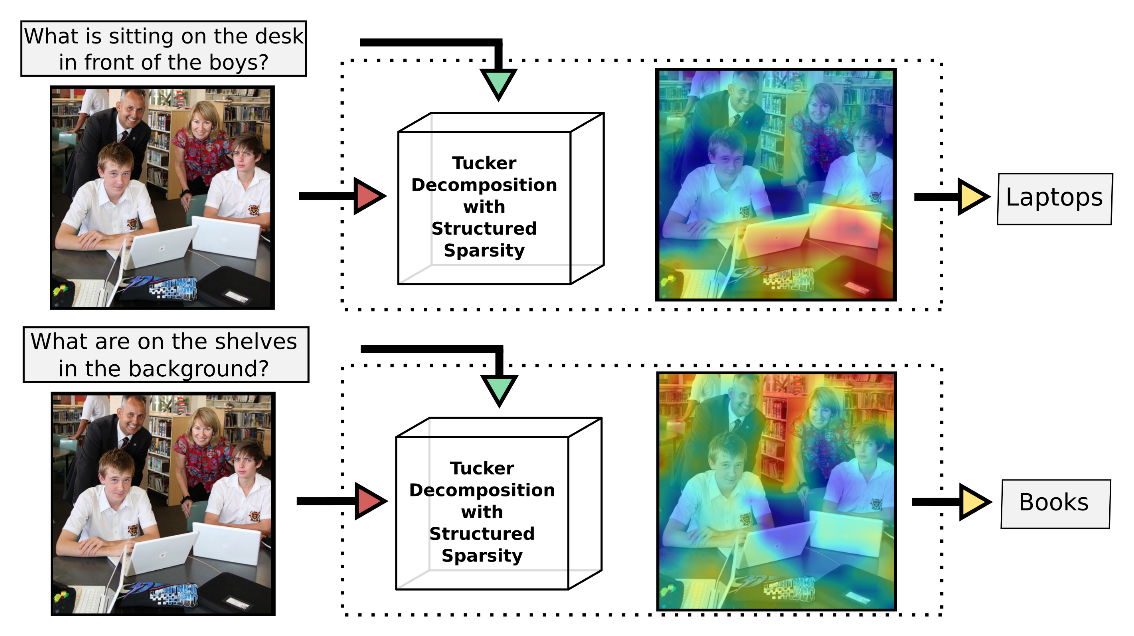
\includegraphics[scale=0.31]{data/mutan_vqa_intro}
\end{frame}
}

{%
% Since Tucker decomposition is a way to approximate a tensor with a lower-rank
% tensor, this image of a clown approximated with SVD is used to illustrate the
% amount of information that can be retained while reducing dimensionality.
% The image, originally 200x320, has been approximated with a rank 20 matrix
% and therefore gone from 200x320 = 64000 numbers to (200 + 320 + 1)x20 = 10420
% numbers.
\setbeamertemplate{frame footer}{\cite{Murphy:2012:MLP:2380985}}
\begin{frame}{Low rank tensor approximations}
        \center{}
        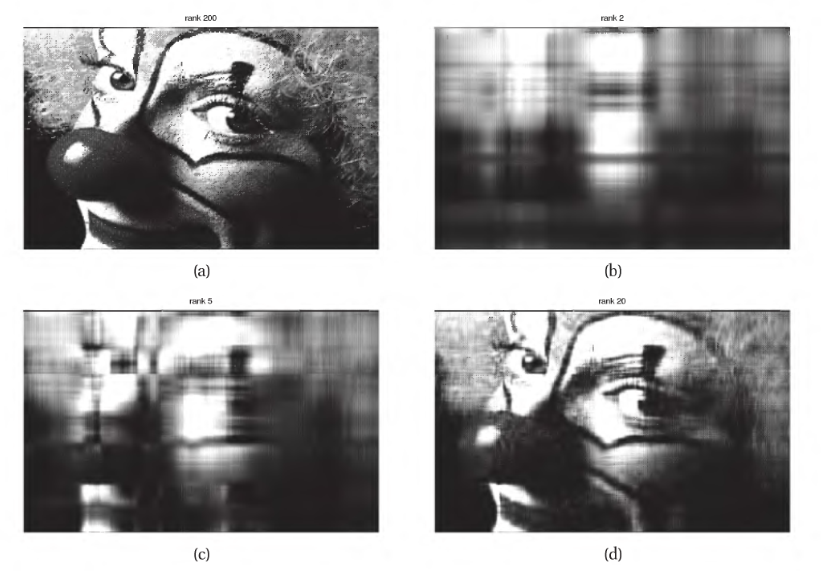
\includegraphics[scale=0.35]{data/low_rank_clown}
\end{frame}
}

{%
% Tucker decomposition is also called higher-order Principal Components
% Analysis. This image is to visualize the PCA projection of D = 2 data to
% an L = 1 space. The points have been projected onto the eigenvector of
% highest eigenvalue, which is also the line of highest covariance between the
% D dimensions.
\setbeamertemplate{frame footer}{\cite{Murphy:2012:MLP:2380985}}
\begin{frame}{PCA}
        \center{}
        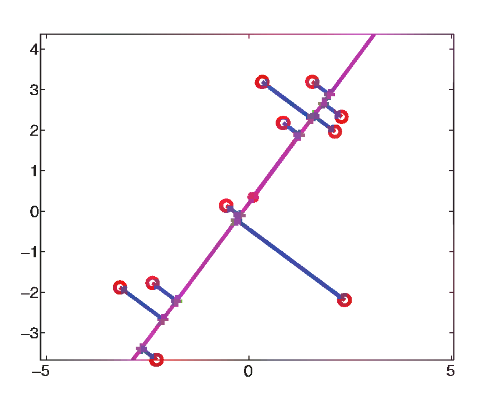
\includegraphics[scale=0.4]{data/pca}
\end{frame}
}

{%
% Fibers needed for explanation of mode-i tensor product used in Tucker
% decomposition, which is the fusion operator in the MUTAN model.
\setbeamertemplate{frame footer}{\cite{Kolda:2009:TDA:1655228.1655230}}
\begin{frame}{Tensor mode-$i$ fibers}
        \center{}
        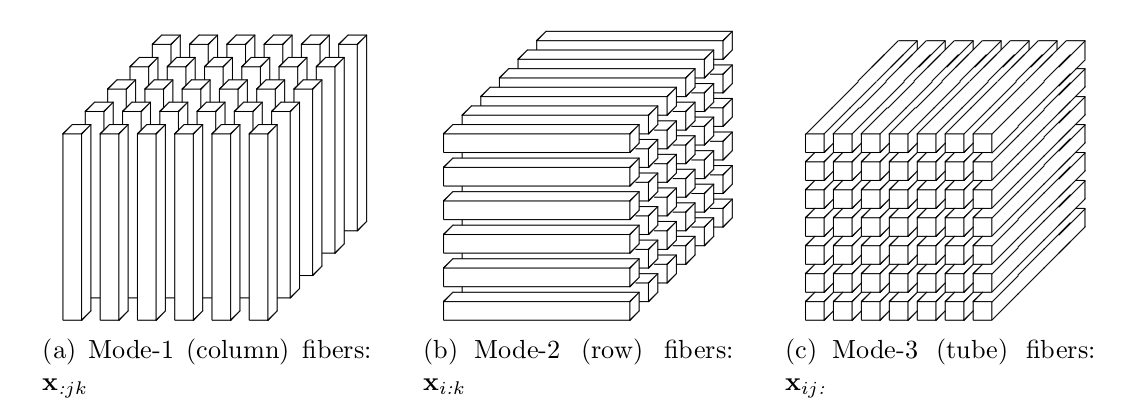
\includegraphics[scale=0.275]{data/tensor_fibers}
\end{frame}
}

{%
% This slide is to illustrate dimensionality reduction in the tensor product.
% In this case, mode-3 tensor multiplication between a 3D tensor and a vector
% reduces a K dimension down to 1 dimension.
%
% In general, an n-mode tensor product of a tensor X with a matrix will reduce
% the nth dimension of the tensor to the number of rows of the matrix, which is
% what is happening in the Tucker decomposition.
\begin{frame}{Tensor product}
        \center{}
        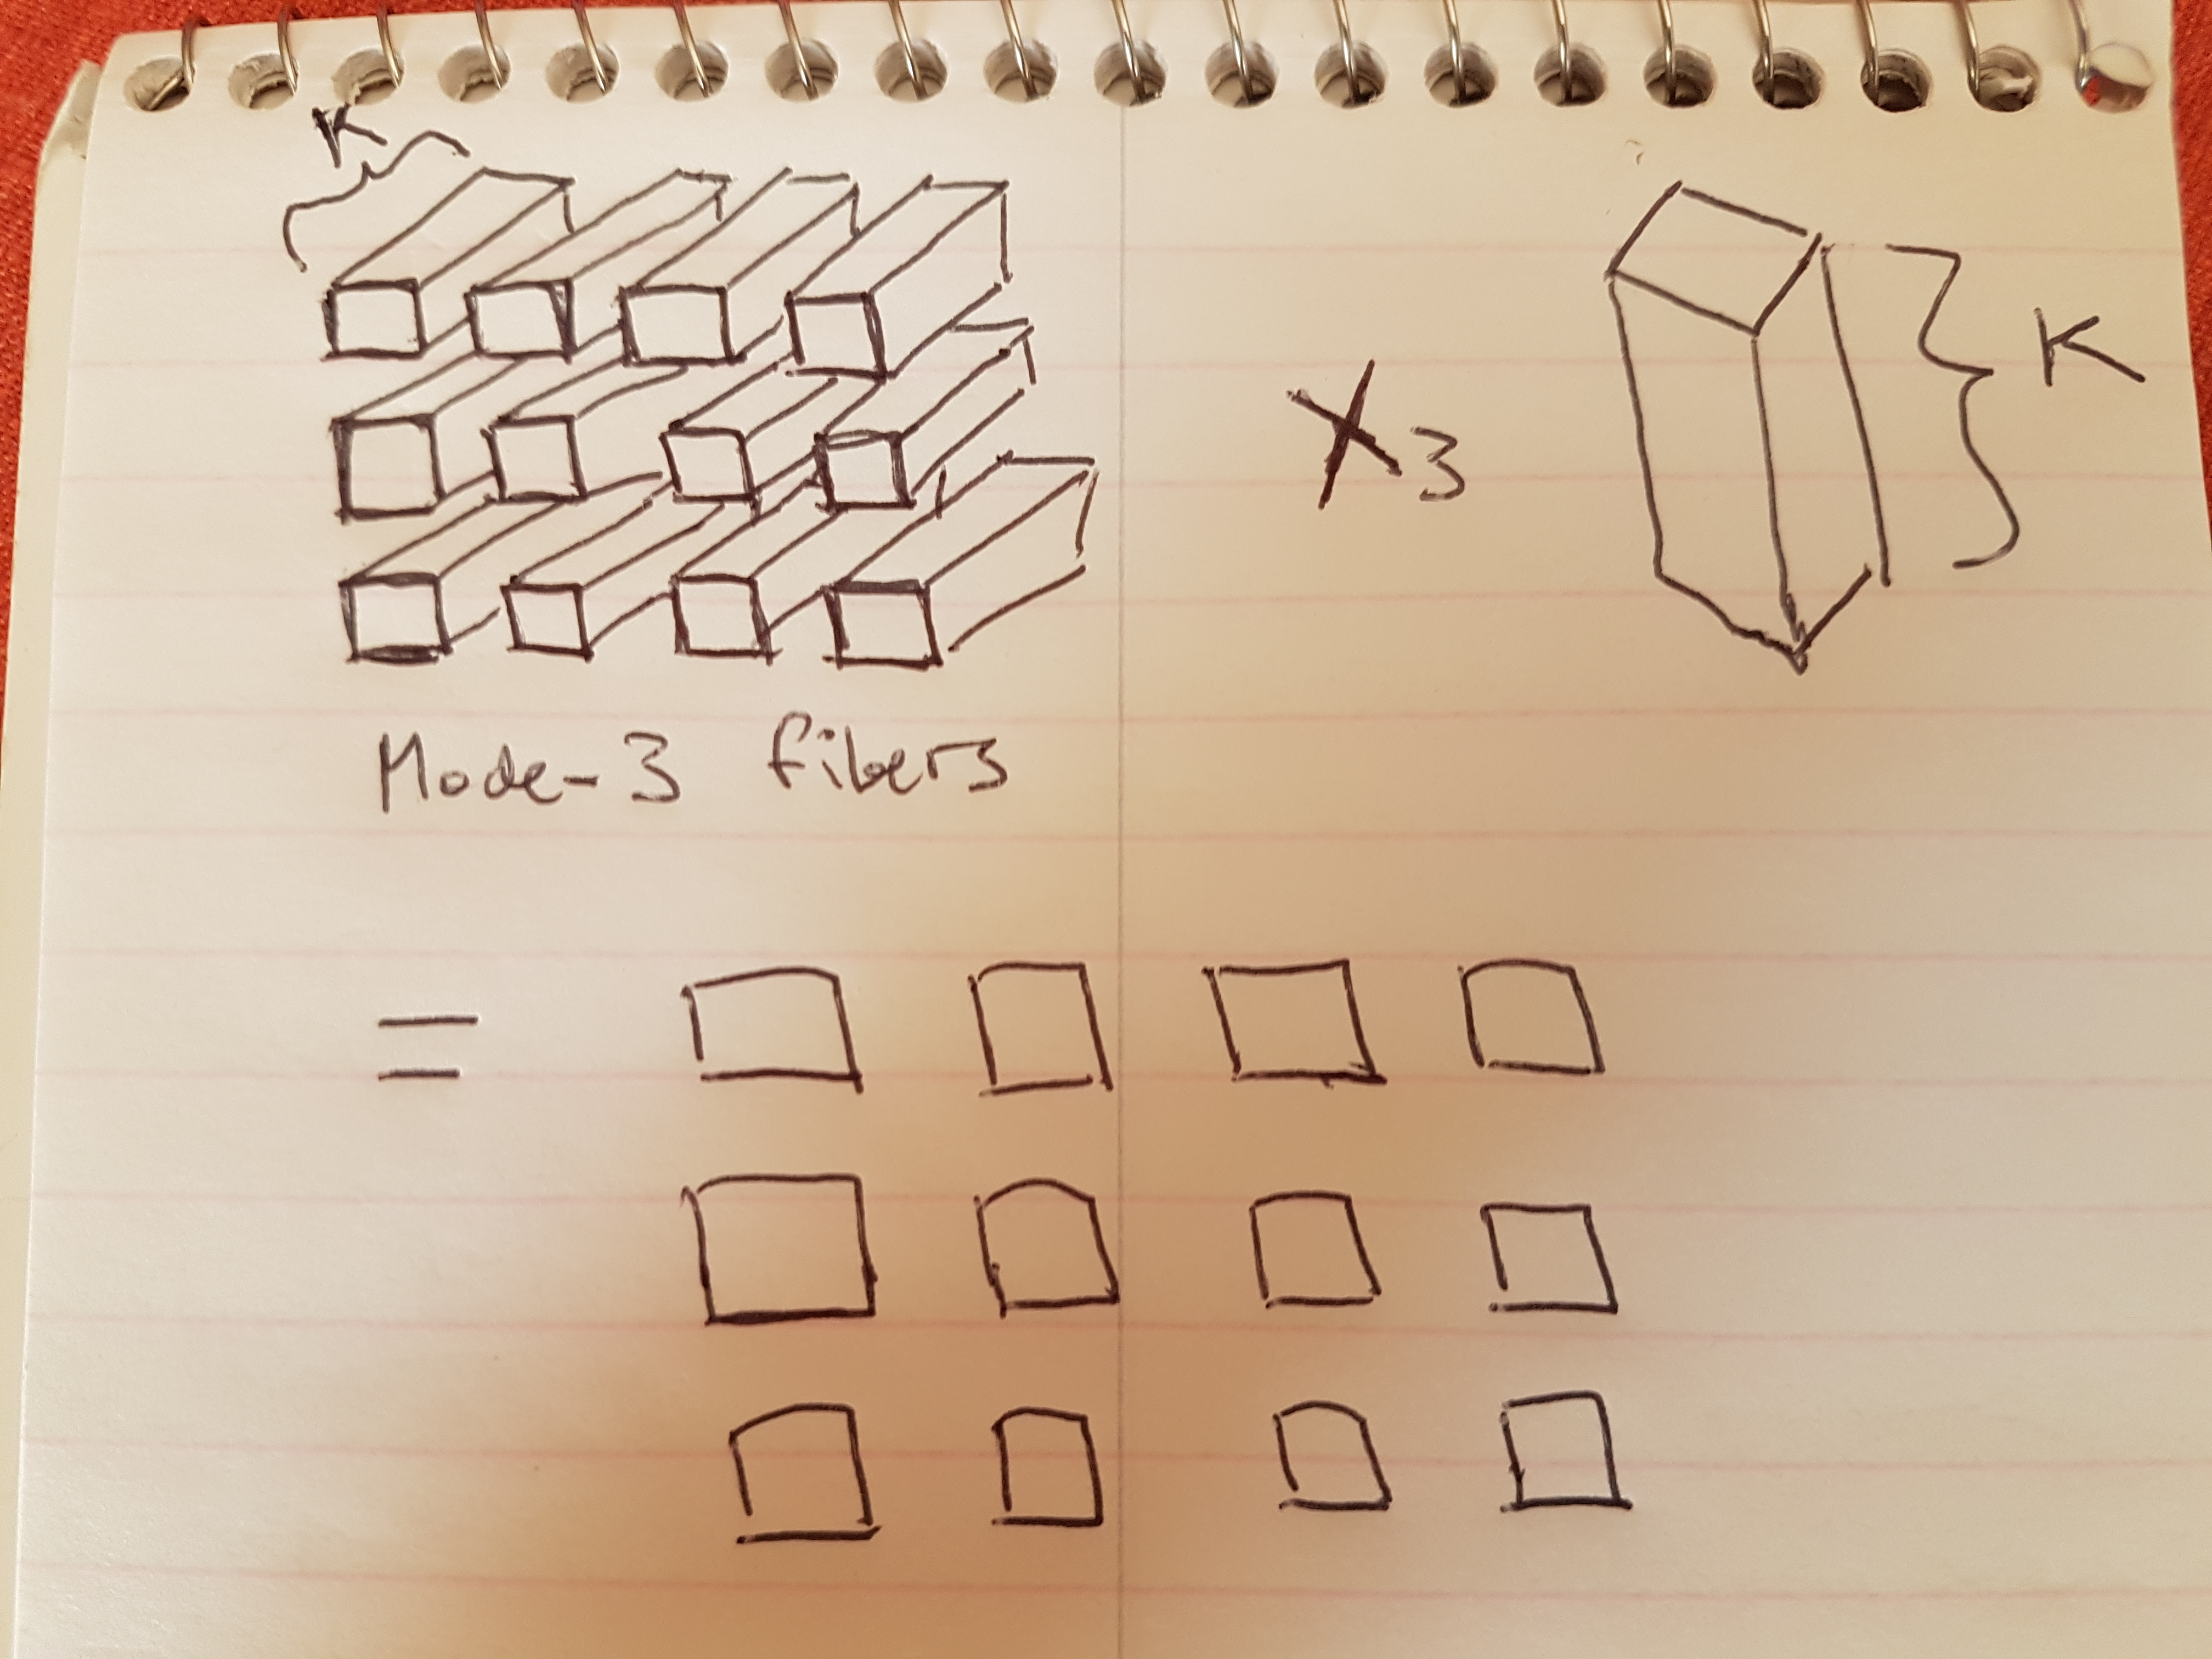
\includegraphics[scale=0.075]{data/tensor_product}
\end{frame}
}

{%
% This is the Tucker decomposition used as the multi-modal fusion operator in
% MUTAN. Here the matrices A, B and C are analogous to the principal components
% eigenvectors in PCA.
\setbeamertemplate{frame footer}{\cite{Kolda:2009:TDA:1655228.1655230}}
\begin{frame}{Tucker decomposition}
        \center{}
        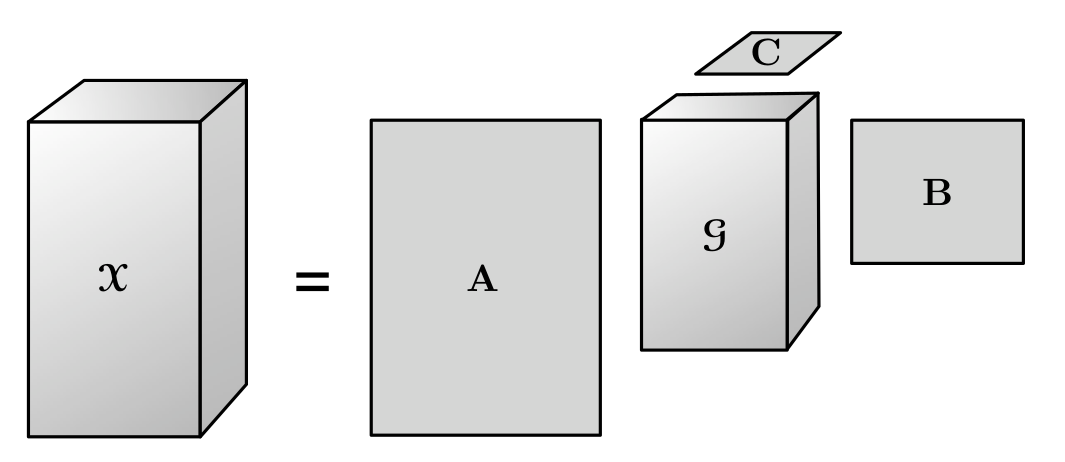
\includegraphics[scale=0.28]{data/tucker_decomp}
        \begin{equation*}
                \mathcal{X} \approx \mathcal{G} \times_1 \mathbf{A} \times_2 \mathbf{B} \times_3 \mathbf{C}
        \end{equation*}
\end{frame}
}

{%
% Here, the outer-product, or "bilinear" relationship, between the sentence
% embedding q and the image embedding v is approximated using the Tucker
% decomposition.
\setbeamertemplate{frame footer}{\cite{DBLP:journals/corr/Ben-younesCCT17}}
\begin{frame}{MUTAN}
        \center{}
        \hspace*{-1.0cm}
        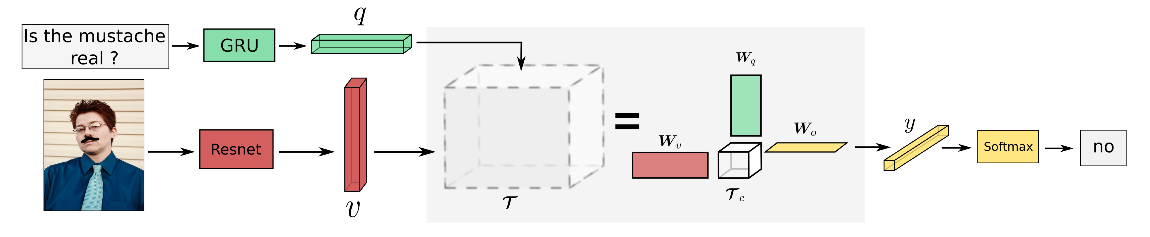
\includegraphics[scale=0.31]{data/mutan}
        \begin{equation*}
                y = \left(\left(\mathcal{T}_c \times_1 \left(\mathbf{q}^T\mathbf{W}_q\right)\right)
                        \times_2 \left(\mathbf{v}^T\mathbf{W}_v\right)\right)
                    \times_3 \mathbf{W}_o
        \end{equation*}
\end{frame}
}

{%
% Contrast of the Tucker decomposition with Multimodal Compact Bilinear (MCB)
% and Multimodal Low-rank Bilinear (MLB).
%
% On the val split of the VQA dataset, the full MUTAN method achieved
% performance of 58.16 overall as compared with the next best result, 57.94
% from MLB, and compared with 56.92 from a baseline that just concatenates v
% and q.
\setbeamertemplate{frame footer}{\cite{DBLP:journals/corr/Ben-younesCCT17}}
\begin{frame}{MCB vs. MLB vs. MUTAN}
        \center{}
        \hspace*{-0.9cm}
        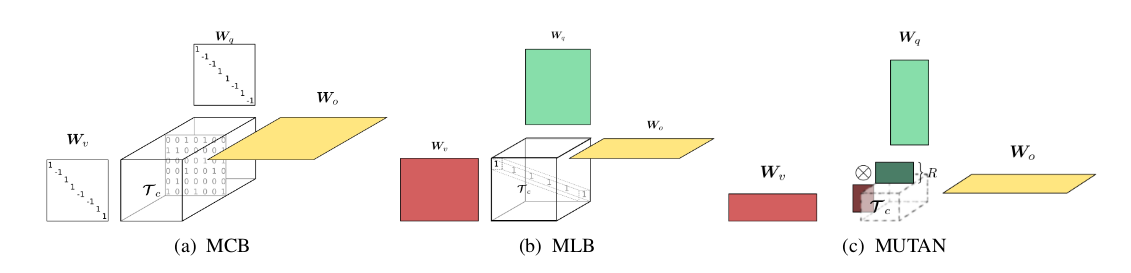
\includegraphics[scale=0.31]{data/mcb_mlb_mutan}
\end{frame}
}

{%
% Winner of Kinetics challenge.
% Uses L2-normalization followed by concatenation as their fusion operator.
\setbeamertemplate{frame footer}{\cite{2017arXiv170803805B}}
\begin{frame}{Multi-group shifting attention network}
        \center{}
        \vspace{-0.8cm}
        \hspace*{-0.9cm}
        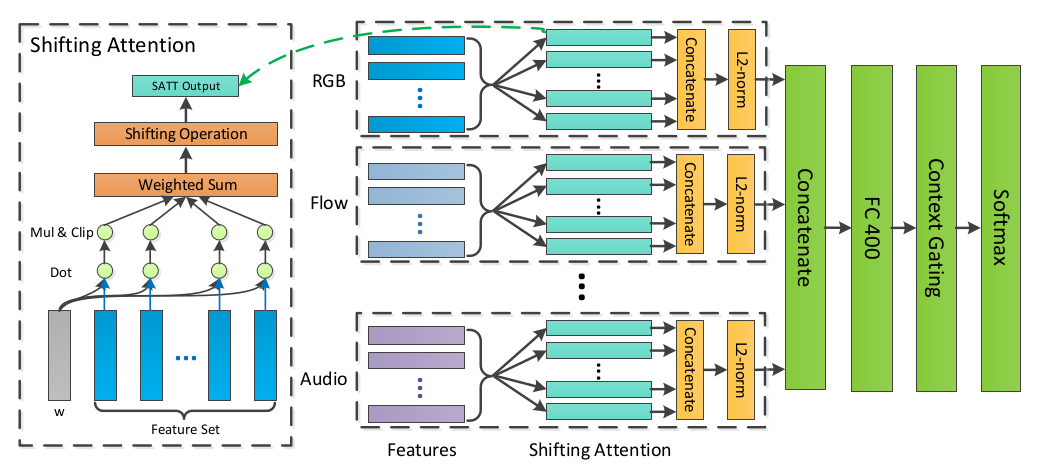
\includegraphics[scale=0.34]{data/multi_group_shifting_attn}
\end{frame}
}

% TODO(brendan): More use-cases from Dhanesh's literature review?

% TODO(brendan): Related work from group (ModOut).


\section{Neural Architecture Search}

{%
% Two problems with REINFORCE as written: variance and convergence.
% Variance can be improved by:
%
%       1. Causality: in the sum, only sum from t' = t to T. Then r(tau) become
%          the "reward-to-go" or q-function. This reduces the magnitude of the
%          term and hence the variance.
%
%       2. Baseline (or REINFORCE comparison): subtract average reward to
%          center the rewards. This does not change the expected value of the
%          policy gradient.
%
%          Optimal variance reduction is b = E[g(tau)^2*r(tau)]/E[g(tau)^2].
%
%       Number of samples can be improved with importance sampling, Trust
%       Region Policy Optimization...
\setbeamertemplate{frame footer}{\cite{deep-rl-berkeley}}
\begin{frame}{REINFORCE overview}
        \vspace{-0.8cm}
        \hspace*{-1.0cm}
        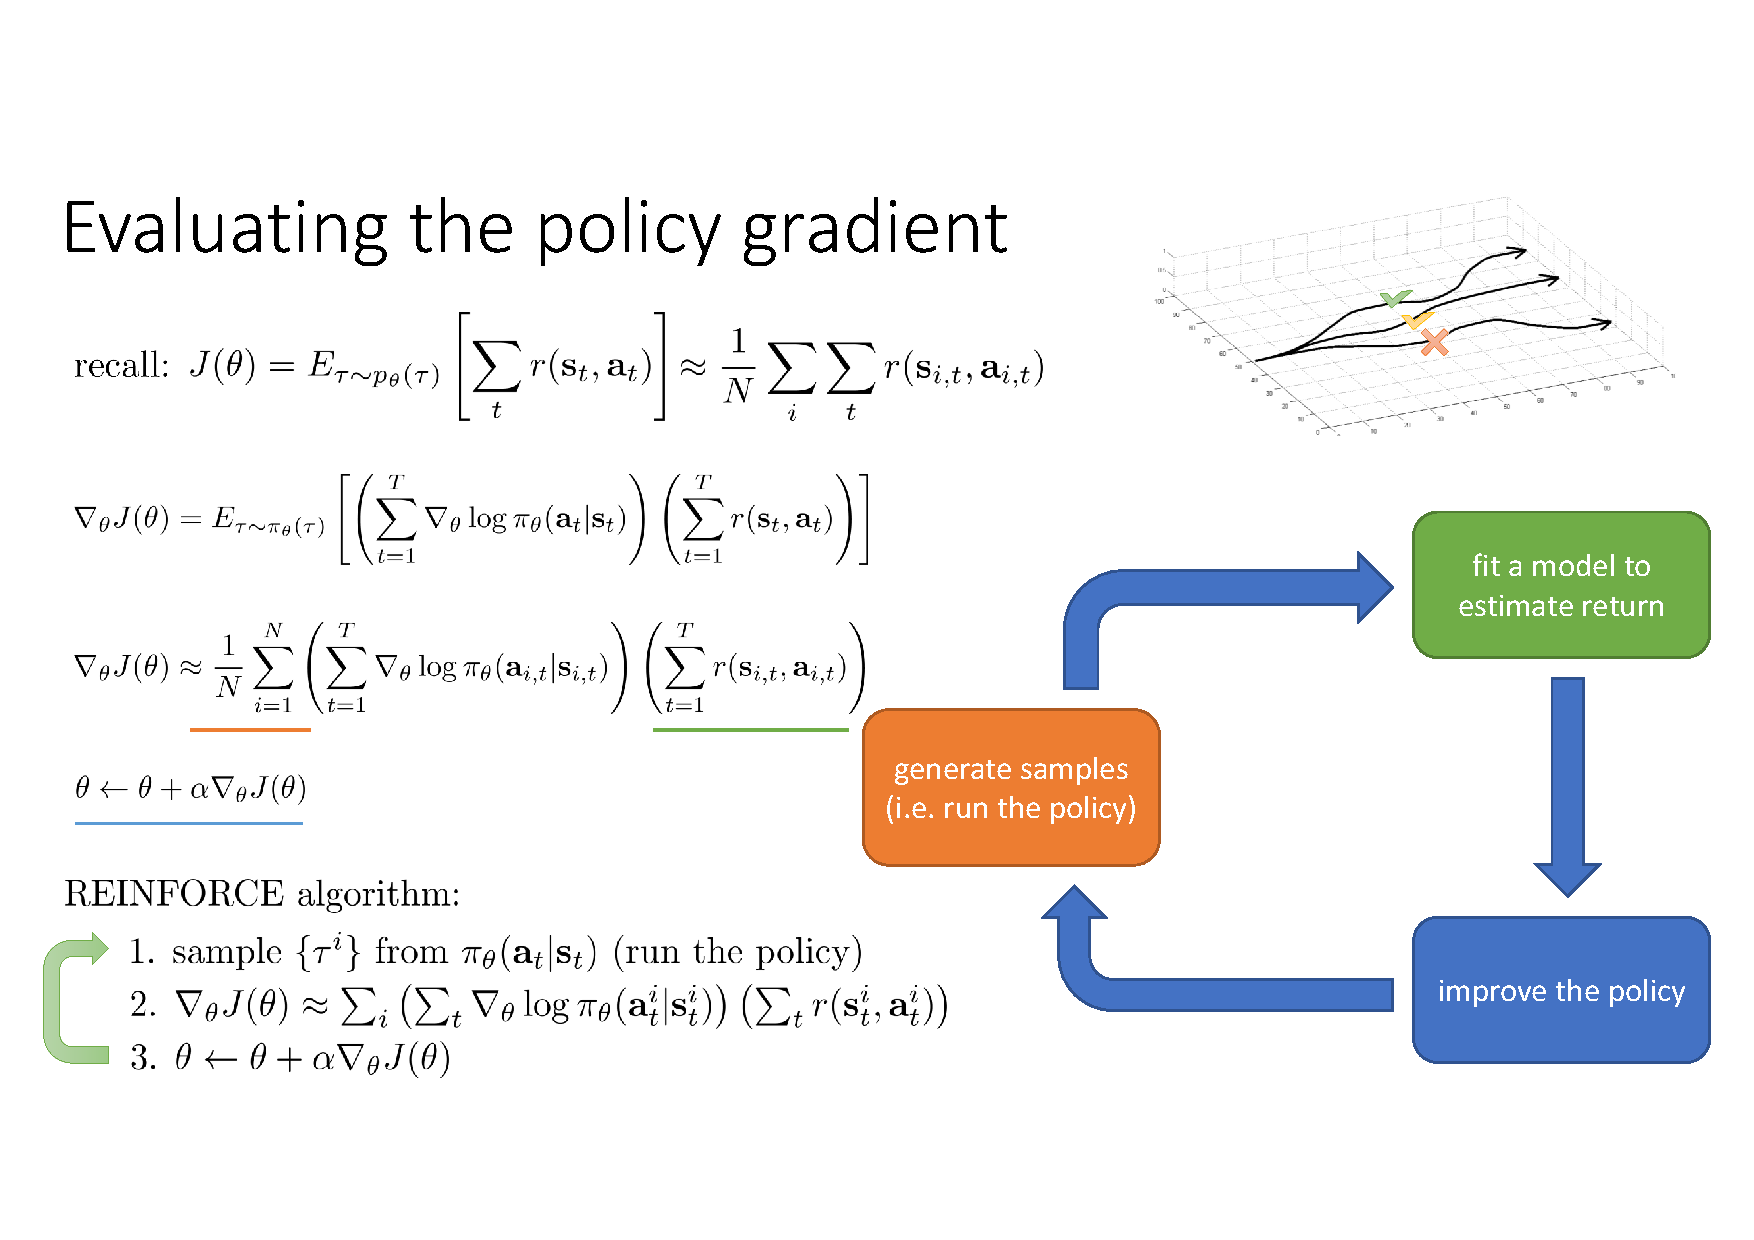
\includegraphics[scale=0.43]{data/reinforce_overview}
\end{frame}
}

{%
\setbeamertemplate{frame footer}{\cite{neural-optimizer-search-46114}}
\begin{frame}{Neural optimizer search overview}
        \center{}
        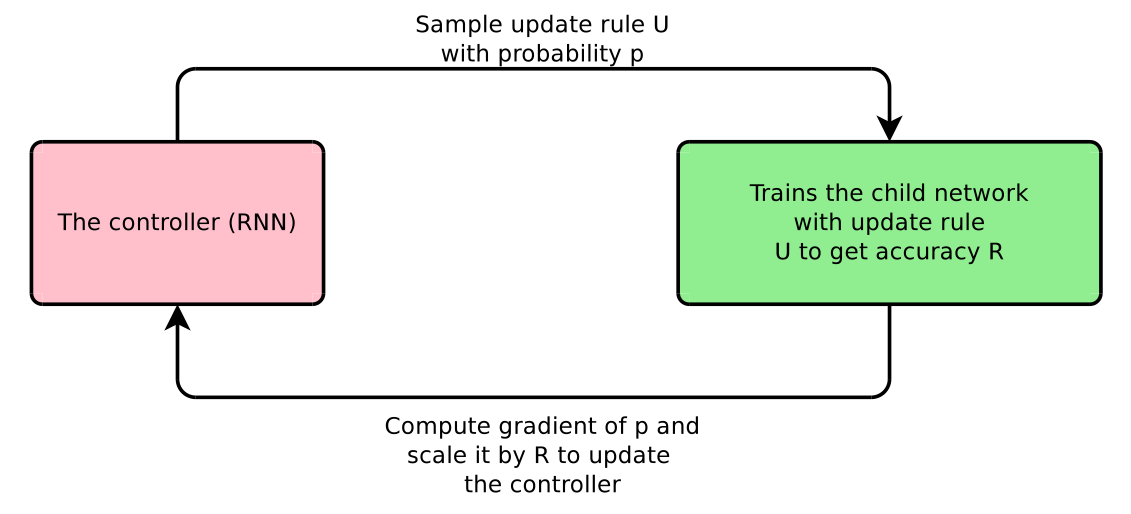
\includegraphics[scale=0.275]{data/neural_arch_update}
\end{frame}
}

{%
% These are common optimizers expressed in the neural optimizer search DSL, to
% illustrate how the search works. The update rules are expressed as a sequence
% of binary operators operating on unary operations. v-hat is a moving average
% of the squared gradients, and m-hat is a moving average of the gradients.
\setbeamertemplate{frame footer}{\cite{neural-optimizer-search-46114}}
\begin{frame}{Common optimizers expressed in DSL}
        \center{}
        \hspace*{-1.0cm}
        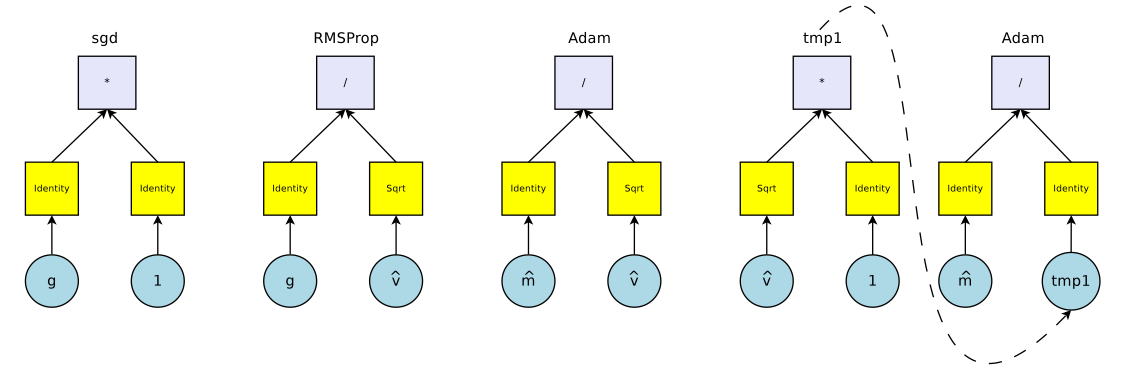
\includegraphics[scale=0.32]{data/common_opts}
\end{frame}
}

{%
% A visualization of the controller outputs.
% In this case, the controller reward plateau'ed after about 15000 sampled
% optimizers.
\setbeamertemplate{frame footer}{\cite{neural-optimizer-search-46114}}
\begin{frame}{Controller RNN overview}
        \center{}
        \hspace*{-1.0cm}
        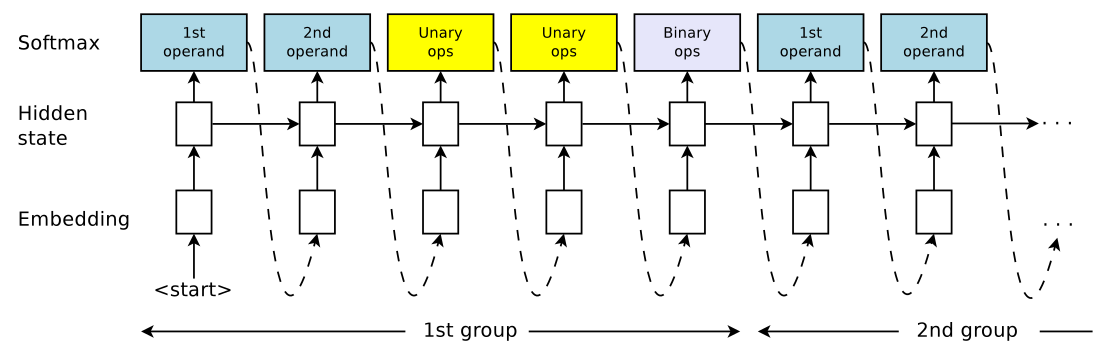
\includegraphics[scale=0.32]{data/neural_opt_controller}
\end{frame}
}

{%
% 10^-3w is (small, constant) white-noise.
% g*e^{sign(g)*sign(m_hat)} decreases the magnitude of the gradient when its
% sign disagrees with the sign of the momentum (moving average of gradient).
% Hence this is an intuitive update rule invented by the controller.
\setbeamertemplate{frame footer}{\cite{neural-optimizer-search-46114}}
\begin{frame}{Generated neural optimizer results}
        \center{}
        \begin{tabular}{l r}
                \emph{Optimizer} & \emph{Best Test} \\
                \midrule{}
                SGD & 91.9 \\
                Momentum & 92.3 \\
                ADAM & 90.7 \\
                RMSProp & 90.3 \\
                \midrule{}
                $[e^{\textrm{sign}(g)*\textrm{sign}(\hat{m})} + \textrm{clip}(g, 10^{-4})]*g$ & 93.1 \\
                $\textrm{drop}(\hat{m}, 0.3)*e^{10^{-3}w}$ & 93.2 \\
                $g*e^{\textrm{sign}(g)*\textrm{sign}(\hat{m})}$ & 92.8
        \end{tabular}
\end{frame}
}

{%
% A diagram of the action procedure of the RNN controller for creating
% convnets.
% Anchor points take skip connections based on sigmoids of tanh's of weighted
% sums of the previous layer's hidden state and the current (input) layer's
% hidden state.
\setbeamertemplate{frame footer}{\cite{neural-architecture-search-45826}}
\begin{frame}{Neural architecture search: convolutional net}
        \center{}
        \vspace{-1.5cm}
        \hspace*{-1.25cm}
        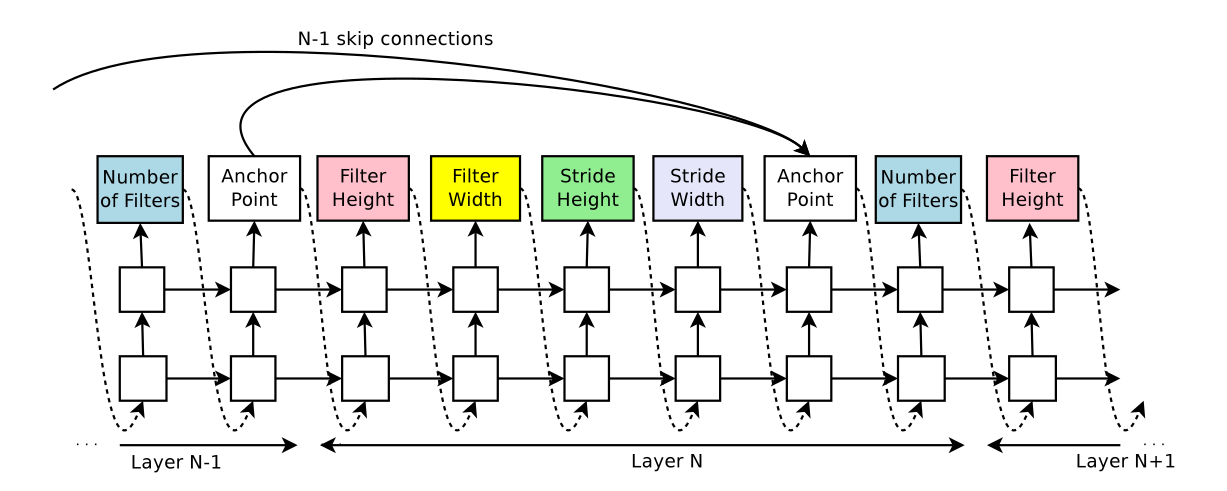
\includegraphics[scale=0.3]{data/neural_arch_convnet}
\end{frame}
}

{%
% RNNs are generalized into a tree structure.
% The RNN controller predicts, for each index of the tree, a binary op and
% unary op (activation), along with tree indices corresponding to the input and
% output cell states (akin to cell state in LSTMs).
% This illustration uses base 2, while the true architectures searched over
% used base 8.
% Search space for RNNs: 6*10^16. 15000 architectures evaluated.
\setbeamertemplate{frame footer}{\cite{neural-architecture-search-45826}}
\begin{frame}{Neural architecture search: RNN}
        \center{}
        \vspace{-1.25cm}
        \hspace*{-1.25cm}
        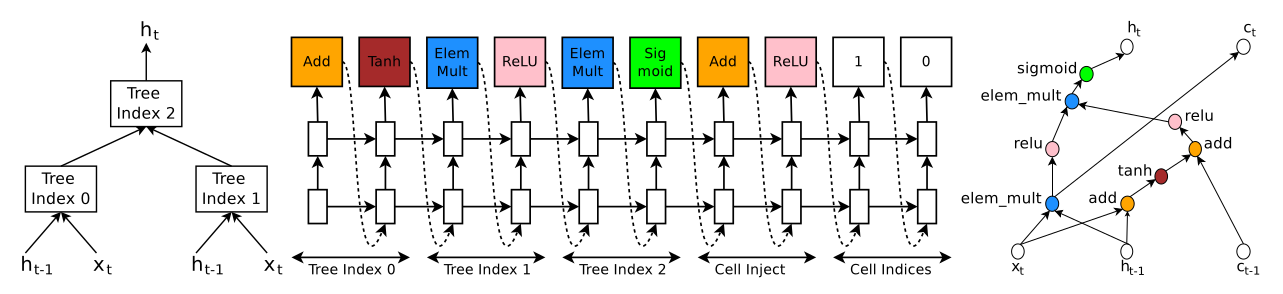
\includegraphics[scale=0.29]{data/neural_arch_rnn}
\end{frame}
}

{%
\setbeamertemplate{frame footer}{\cite{neural-architecture-search-45826}}
\begin{frame}{Generated convolutional net}
        \center{}
        \vspace{-0.25cm}
        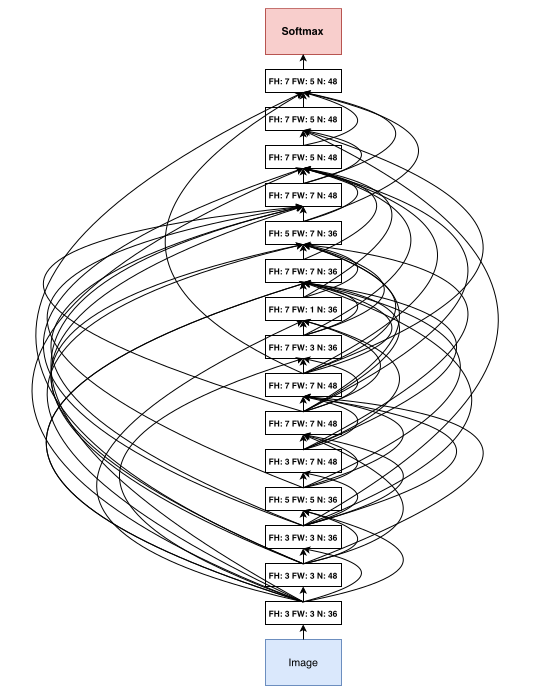
\includegraphics[scale=0.33]{data/neural_arch_convnet_output}
\end{frame}
}

{%
% The top left is an LSTM. The top right and bottom are generated RNNs,
% difference being that on the bottom the controller was allowed to use max and
% sin.
\setbeamertemplate{frame footer}{\cite{neural-architecture-search-45826}}
\begin{frame}{Generated RNN}
        \center{}
        \vspace{-0.25cm}
        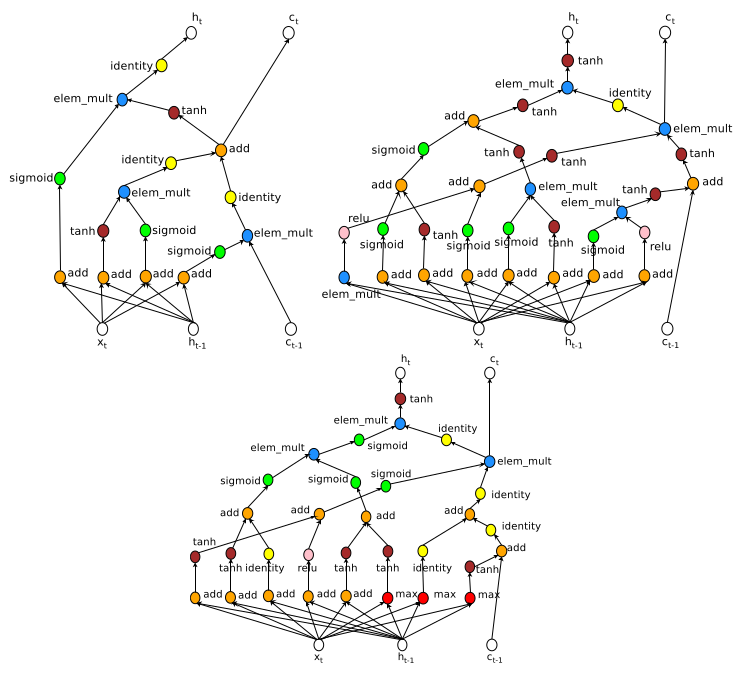
\includegraphics[scale=0.32]{data/neural_arch_rnn_output}
\end{frame}
}


\section{Neural Fusion Operator Search}

\begin{frame}[standout]
        How can the neural architecture search techniques we just learned be
        applied to improve the multi-modal fusion operators we discussed
        earlier?
\end{frame}

{%
% Two extensions:
%
% 1. Is it possible to incorporate the state_i from the reinforcement learning
%    state-action space, where state_i in this case is the current architecture
%    of the network? This would reduce the action space to adding or removing
%    layers.
%
% 2. Add an additional anchor point to predict skip connections to different
%    layers of the optical flow, RGB and audio convnets.
\begin{frame}{Neural search multi-modal extension}
        \center{}
        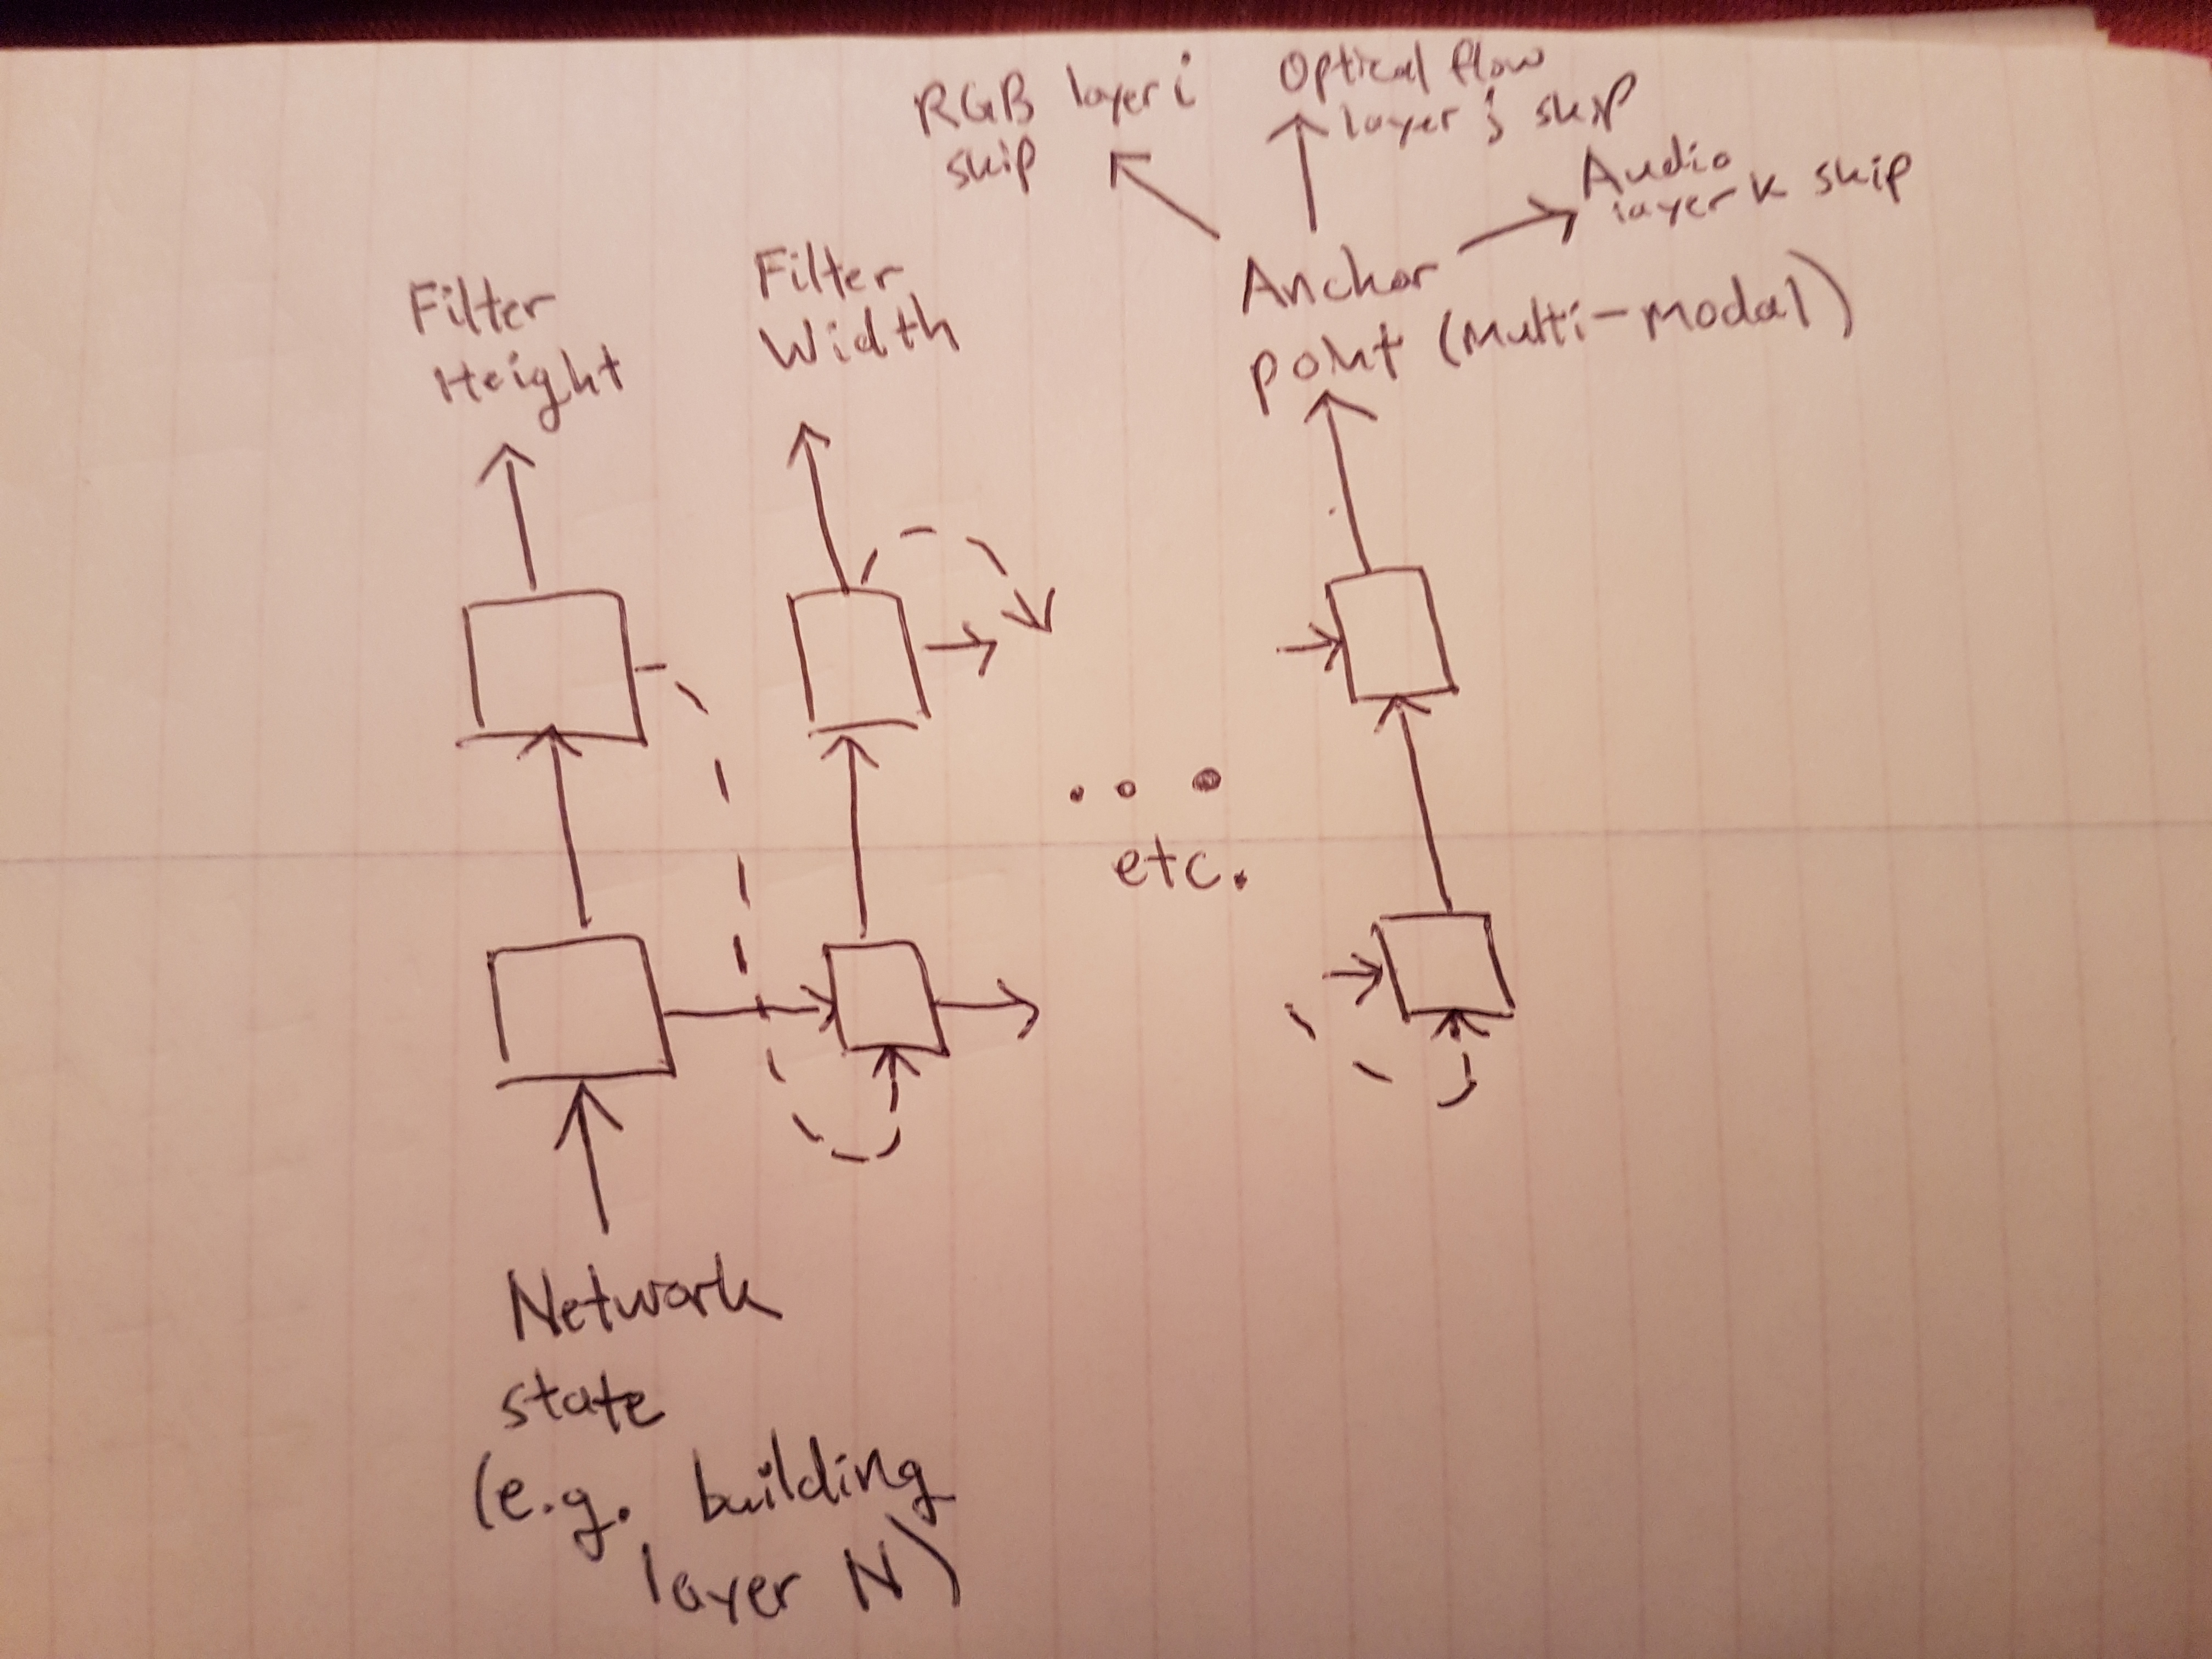
\includegraphics[scale=0.075]{data/multi_modal_neural}
\end{frame}
}


\section{Conclusions}

\begin{frame}[fragile]{Conclusions}
        \begin{itemize}[<+- | alert@+>]
                \item Fusion in VQA by approximating outer-product between
                        embeddings of different modes.

                \item Policy gradient method for neural architecture/optimizer
                        search.

                \item Extension to fusion operator still in early stages.
        \end{itemize}
\end{frame}

\begin{frame}[standout]
        Questions?
\end{frame}

\appendix

\begin{frame}[allowframebreaks]{References}
        \bibliography{fusion-operator}
        \bibliographystyle{apalike}
\end{frame}

\end{document}
